

\documentclass[10pt, a4paper, twocolumn]{article}
%%%%%%%%%%%%%%%%%%%%%%%%%%%%%%%%%%%%%%%%%
% Wenneker Article
% Structure Specification File
% Version 1.0 (28/2/17)
%
% This file originates from:
% http://www.LaTeXTemplates.com
%
% Authors:
% Frits Wenneker
% Vel (vel@LaTeXTemplates.com)
%
% License:
% CC BY-NC-SA 3.0 (http://creativecommons.org/licenses/by-nc-sa/3.0/)
%
%%%%%%%%%%%%%%%%%%%%%%%%%%%%%%%%%%%%%%%%%

%----------------------------------------------------------------------------------------
%	PACKAGES AND OTHER DOCUMENT CONFIGURATIONS
%----------------------------------------------------------------------------------------

\usepackage[english]{babel} % English language hyphenation

\usepackage{microtype} % Better typography

\usepackage{amsmath,amsfonts,amsthm} % Math packages for equations

\usepackage[svgnames]{xcolor} % Enabling colors by their 'svgnames'

\usepackage[hang, small, labelfont=bf, up, textfont=it]{caption} % Custom captions under/above tables and figures

\usepackage{booktabs} % Horizontal rules in tables

\usepackage{lastpage} % Used to determine the number of pages in the document (for "Page X of Total")

\usepackage{graphicx} % Required for adding images

\usepackage{enumitem} % Required for customising lists
\setlist{noitemsep} % Remove spacing between bullet/numbered list elements

\usepackage{sectsty} % Enables custom section titles
\allsectionsfont{\usefont{OT1}{phv}{b}{n}} % Change the font of all section commands (Helvetica)

\usepackage{mathtools, verbatim, fancyhdr, chngcntr, algorithm, algorithmic}
\usepackage[colorlinks=true,linkcolor=black, citecolor=blue]{hyperref}

%	MARGINS AND SPACING
%----------------------------------------------------------------------------------------

\usepackage{geometry} % Required for adjusting page dimensions

\geometry{
	top=1cm, % Top margin
	bottom=1.5cm, % Bottom margin
	left=2cm, % Left margin
	right=2cm, % Right margin
	includehead, % Include space for a header
	includefoot, % Include space for a footer
	%showframe, % Uncomment to show how the type block is set on the page
}

\setlength{\columnsep}{7mm} % Column separation width

%----------------------------------------------------------------------------------------
%	FONTS
%----------------------------------------------------------------------------------------

\usepackage[T1]{fontenc} % Output font encoding for international characters
\usepackage[utf8]{inputenc} % Required for inputting international characters

\usepackage{XCharter} % Use the XCharter font

%----------------------------------------------------------------------------------------
%	HEADERS AND FOOTERS
%----------------------------------------------------------------------------------------

\usepackage{fancyhdr} % Needed to define custom headers/footers
\pagestyle{fancy} % Enables the custom headers/footers

\renewcommand{\headrulewidth}{0.0pt} % No header rule
\renewcommand{\footrulewidth}{0.4pt} % Thin footer rule

\renewcommand{\sectionmark}[1]{\markboth{#1}{}} % Removes the section number from the header when \leftmark is used

%\nouppercase\leftmark % Add this to one of the lines below if you want a section title in the header/footer

% Headers
\lhead{} % Left header
\chead{\textit{\thetitle}} % Center header - currently printing the article title
\rhead{} % Right header

% Footers
\lfoot{} % Left footer
\cfoot{} % Center footer
\rfoot{\footnotesize Page \thepage\ of \pageref{LastPage}} % Right footer, "Page 1 of 2"

\fancypagestyle{firstpage}{ % Page style for the first page with the title
	\fancyhf{}
	\renewcommand{\footrulewidth}{0pt} % Suppress footer rule
}
\setlength\parindent{0pt} % for not indenting

%----------------------------------------------------------------------------------------
%	TITLE SECTION
%----------------------------------------------------------------------------------------

\newcommand{\authorstyle}[1]{{\large\usefont{OT1}{phv}{b}{n}\color{DarkRed}#1}} % Authors style (Helvetica)

\newcommand{\institution}[1]{{\footnotesize\usefont{OT1}{phv}{m}{sl}\color{Black}#1}} % Institutions style (Helvetica)

\usepackage{titling} % Allows custom title configuration

\newcommand{\HorRule}{\color{DarkGoldenrod}\rule{\linewidth}{1pt}} % Defines the gold horizontal rule around the title

\pretitle{
	\vspace{-30pt} % Move the entire title section up
	\HorRule\vspace{10pt} % Horizontal rule before the title
	\fontsize{32}{36}\usefont{OT1}{phv}{b}{n}\selectfont % Helvetica
	\color{DarkRed} % Text colour for the title and author(s)
}

\posttitle{\par\vskip 15pt} % Whitespace under the title

\preauthor{} % Anything that will appear before \author is printed

\postauthor{ % Anything that will appear after \author is printed
	\vspace{10pt} % Space before the rule
	\par\HorRule % Horizontal rule after the title
	\vspace{20pt} % Space after the title section
}

%----------------------------------------------------------------------------------------
%	ABSTRACT
%----------------------------------------------------------------------------------------

\usepackage{lettrine} % Package to accentuate the first letter of the text (lettrine)
\usepackage{fix-cm}	% Fixes the height of the lettrine

\newcommand{\initial}[1]{ % Defines the command and style for the lettrine
	\lettrine[lines=3,findent=4pt,nindent=0pt]{% Lettrine takes up 3 lines, the text to the right of it is indented 4pt and further indenting of lines 2+ is stopped
		\color{DarkGoldenrod}% Lettrine colour
		{#1}% The letter
	}{}%
}

\usepackage{xstring} % Required for string manipulation

\newcommand{\lettrineabstract}[1]{
	\StrLeft{#1}{1}[\firstletter] % Capture the first letter of the abstract for the lettrine
	\initial{\firstletter}\textit{\StrGobbleLeft{#1}{1}} % Print the abstract with the first letter as a lettrine in italic
}

% %----------------------------------------------------------------------------------------
% %	BIBLIOGRAPHY
% %----------------------------------------------------------------------------------------
\makeatletter
\def\@biblabel#1{[#1]} % not to show names in "thebibliography" environment. If not, put "[#1]" inside {}
\makeatother

% \usepackage[backend=bibtex,style=authoryear,natbib=true]{biblatex} % Use the bibtex backend with the authoryear citation style (which resembles APA)

% \addbibresource{example.bib} % The filename of the bibliography

% \usepackage[autostyle=true]{csquotes} % Required to generate language-dependent quotes in the bibliography
 % Specifies the document structure and loads requires packages


\title{Drug reviews: NLP approaches to investigate patients belief}
\author{
	\authorstyle{Greta Gravina and Niccolò Rocchi}
	\newline\newline
	\institution{Università degli Studi di Milano-Bicocca, Milan, Italy}
}

\date{June, 2023} 

% DOCUMENT

\begin{document}

    \maketitle
    \thispagestyle{firstpage} % Apply the page style for the first page (no headers and footers)

    % ABSTRACT

    \lettrineabstract{Natural Language Processing has revealed a powerful tool in Digital Era for shaping human thoughts. In the present work we implemented Topic Modelling and Sentiment Analysis methods for analyzing patients' feelings about drugs. Results suggested LDA and LightGBM as the two finest algorithms for obtaining valuable information.}\\
    
    %	ARTICLE CONTENTS 
    
    \section{Introduction}
        Being able to interpret human thoughts, or even to formalize it, has been one of the most complex challenges. Modelling language in a mathematical structure, not only provides a synthetic picture of what we think, but also highly valuable reasoning. 
        Text Mining's aim is exactly to interpret and to model huge portions 
        of unstructured human considerations.\\
        In this work we want to approach to this problem, by diving in a clinical reviews data set (see \cite{Graber}). Applying Topic Modelling and Sentiment Analysis techniques, our aim is to model patients feedback in order to reach out precious insights. Making sense of clients feelings, in fact, is often the core of strategical analysis in companies.  

    \section{Objectives}
        The research question we face in this work takes into account \emph{what can we do} for patients. Prescriptive analysis is orders of magnitude harder than a simpler descriptive or predictive analysis. However, we seek to mine text reviews for disclosing which are the actions a pharmaceutical company could do for its clients in order to improve their condition. Our focus is on negative aspects the patients found in their therapies, hence we apply Topic Modelling techniques. We also aim to understand \emph{how patients feel} about drugs through discriminating reviews by the use of Text Classification Sentiment Analysis.
        

    \section{Related work}
        Although an increasing importance is given day by day to NLP approaches in Health Care, just a few scientific articles have analyzed drug reviews. Specifically, the application of topic modelling seems not to be a tendency among drug reviews, while it is among e-commerce reviews, for example. Our main reference in applying topic modelling is \cite{drug}. In particular they suggest how to properly balance data before applying models, following then a data driven process. They also make use of Structural Topic Model algorithm, comparing it to Latent Dirichlet Allocation (\cite{LDA}). Indeed, while LDA --- or other models that extended this, such as Correlated Topic Model --- is currently used as one of the more suitable topic model in every field and supported by large part of literature, STM is relatively a new approach, although it has been applied in political sciences and linguistics. The adoption of STM in this work is also motivated by \cite{hotel}. They state that: ``\textit{Limitations of LDA and nature of customer reviews make LDA not feasible for the extraction of customer dissatisfaction}''.\\
        
        Text Classification of reviews based on Sentiment Analysis is a technique used to analyze and categorize sentences and reviews as positive, negative, or neutral based on the sentiment conveyed in the text (\cite{Kaggle_choco, Kaggle_Peter}).
        Sentiment Analysis involves the use of natural language processing techniques and machine learning algorithms to identify the emotional tone of the text, such as whether it expresses positive, negative, or neutral sentiment towards a particular drug. Nowadays, this approach can be useful for pharmaceutical companies, healthcare providers, and patients to understand consumer opinions and attitudes towards different drugs, \cite{drug2} . It can also help in identifying potential adverse effects and issues related to drug efficacy and patient compliance, as we can observe in some related works.
        
    \section{Data preparation}
        The so called J-curve is particularly common in online ratings systems. The typical U-shaped distribution of ratings - in this case from $1$ to $10$ - is the evidence of a self-selection bias called \emph{under reporting}: only the reviewers who feel strongly about a product are likely to review that product, whenever positively or not. Input data quality is fundamental to make sense of our Topic Modelling and Sentiment Analysis results and not to be biased. For this reason, for both the models we perform the same data pre-processing. Firstly, we filter out central reviews, i.e. these which rating ranges from $5$ to $8$. We think in fact that topics related to these reviews may not be clearly defined. We then obtain polarized reviews: either very negative or very positive. This is also suggested by \cite{drug} and continuing following their work we balance data in order to have an equal number of positive and negative reviews. Nevertheless, this is not done in an absolute manner, but balancing documents among each drug class. Since original data set does not contain drug type each review refers to, we try to enrich data by matching drug - class pairs with a web scraping strategy. This is done leveraging the fact the data set derives from \cite{drugs.com} site. At a first glance this is a difficult task to be accomplished, given that medication and condition of each patient is hand written by a doctor and not strictly referred to a shared vocabulary. Since not all drugs have been associated with their class, we decide to exclude those records. We also keep the classes that count more than $1000$ reviews, and these are: anorexiants, antidepressants, antimigraine agents, antipsychotics, cns stimulants, contraceptives, GABA (gamma aminobutyric acid analogs), incretin mimetics, laxatives, analgesics, anxiolytics (jointed with sedatives and hypnotics in an unique category), nonsteroidal anti inflammatory agents, skeletal muscle relaxants, smoking cessation agents. Notice that grouping by class is less fine-grained than grouping by medical condition, and more general than grouping by single drug names.
        
    \section{Topic modelling}
        \subsection{Pre-processing}
            Each text document (the review) is been lowered and then tokenized by the Python Natural Language Toolkit. Each token is kept only if completely alphabetic, excluding common drugs information such as number of pills, day of the week and punctuation expressing personal emotions. Next, stop words are removed and each token is stemmed by Porter Stemmer; lemmatization was not applied (see  Section \ref{subsec:top_mod_evaluation} for details). Afterwards we build a word dictionary together with their absolute frequency, filter common and rare words (lower and upper thresholds: $5\%$, $55\%$) and a Bag of Words matrix is created for each document. These will be the inputs for LDA and STM models.
            
        \subsection{Models}
            Among a large collection of topic modelling algorithms, we decide to isolate a count-based and Bayesian approach, both in its base and in a more advanced form: Latent Dirichlet Allocation (LDA) and Structural Topic Modelling (STM). The former is trained using the Python library \texttt{gensim}, while the latter the R package \texttt{stm}. For each one, several runs with different topic number is performed and the best model is chosen based on the best value of a certain cohesion measure. Notice that \emph{the best} here doesn't necessary imply \emph{the highest}, but it refers to the highest accordingly to the elbow method. When the function reaches a local maximum pleateau, and it increases by a little quantity, this is chosen as the best cohesion.\\
            We decide to focus on this type of measure because focusing on perplexity may not yield to human interpretable topics. In contrast, we wish for precise and well separated patients arguments. For their well separation we must rely on some diversity metric, which will be searched and evaluate after having chosen the best model. For both algorithms the best topic number turned up to be 7. Unfortunately, the two packages don't provide the same topic measures, thus the best value is chosen based on CV coherence for LDA (see \cite{Syed}) and on Semantic Coherence for STM (see \cite{Mimno}).\\

            LDA is currently the state of the art of topic modelling, trying to fix some negative aspects of LSA or pLSA. It has its origins in pLSA but varies from it assuming Dirichlet distribution for both word-topic and topic-document distributions. Indeed the sparsification of topics and words in the model is near to reality and likely to happen in reviews: focusing on extreme ones, the patient will explain very few but significant reasons behind her rating. In addition, each topic will be characterized by a few very specific terms. From Figure \ref{fig:lda_diagram} we can see the model diagram. 
            
            \begin{figure}[!ht]
                \centering
                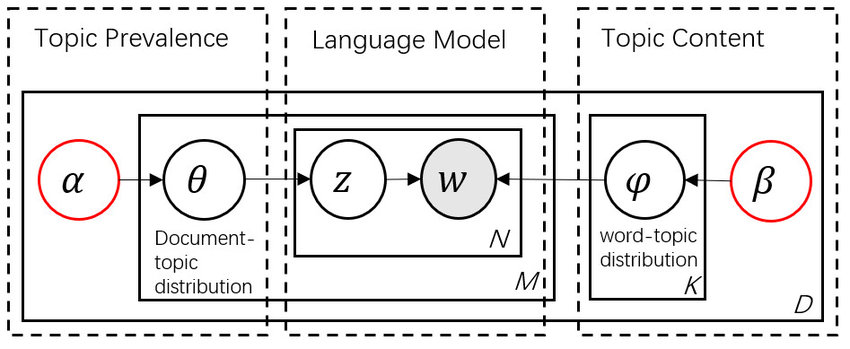
\includegraphics[width = 0.48\textwidth]{LDA_diagram.png}
                \caption{Diagram of Latent Dirichlet Allocation (LDA)}
                \label{fig:lda_diagram}
            \end{figure}

            However, while LDA just learns from documents, the latter also includes in the model other useful covariates. Each review has characteristics of heterogeneity that actually influence it, even if speaking of the same arguments, and we want to include them in the model. This heterogeneity, e.g. people emotions or social background, regard \emph{how} and \emph{how much} a user speaks about each topic. These two aspects influence both topic prevalence --- per document topics distribution --- and topic content --- per topic words distribution ---and are modelled by the insertion of $X$ and $\mu$, which are document-specific covariates. The diagram is shown in Figure \ref{fig:stm_diagram}.
            
            \begin{figure}[!ht]
                \centering
                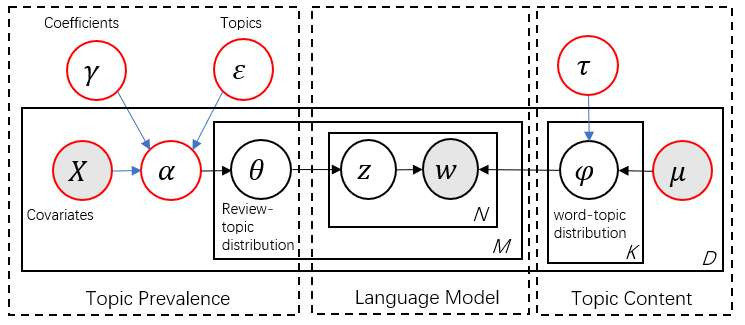
\includegraphics[width = 0.48\textwidth]{STM_diagram.png}
                \caption{Diagram of Structural Topic Modelling (STM)}
                \label{fig:stm_diagram}
            \end{figure}

            The STM model we build includes, as prevalence covariates, a two-values variable representing review positiveness and the year in which it was written, while the context covariate is a categorical variable indicating drug class. 
    
        \subsection{Evaluation}
            \label{subsec:top_mod_evaluation}
            Since it's an unsupervised Machine Learning field, topic modelling task doesn't follow strict rules or metrics in the assessment of its goodness. There is not a specific metric to be optimized, such as a loss function, but there are loads of different approaches for evaluating that model. Speaking about \emph{quantifying} the human judgement, we could isolate two main classes of measures: cohesion and division. High cohesion means the words inside a topic are semantically related (looking at their co-occurrence), bringing us to interpretable topics, while high division ensures that topics speak about different arguments. In this work we focused on cohesion, as already seen: the number of topics is such that maximizes an internal measure of cohesion. However, we want now to evaluate division, since having high cohesion may underlie topics with very frequent and meaningless words. Still, we must rely on different tools provides by the two packages  ---  this is normal, since the two models are structurally different. We could assess a lot of measure or charts, but we decide just to enlighten the most interesting ones.\\
            An other, but more qualitative, possible evaluation looks upon human judgement directly: we could examine topic interpretability, as well as their information or semantic, looking for example at top-$n$ words. We have built two models: every model has 7 topics --- STM also specializes topic words for each drug class --- and for each one we could extract the words based on their relevance. Indeed, relevance is more sophisticated than a simpler occurrence probability and it's defined as: 
            $$\mathbf{Rel}_{\lambda}(\text{word}~w|\text{topic}~t)\coloneqq \lambda p(w|t)+(1-\lambda) \frac{p(w|t)}{p(w)}$$
            Depending on $\lambda$ we decide to give more or less importance to the absolute probability $p(w)$. Optimal values for topic interpratibility are usually $\lambda = 0, 0.6, 1$.\\
            In addition to further considerations, we also make available a very useful interactive intertopic map for LDA, and a shiny app for STM. For instructions on how to use these resources, so that everyone can answer she's own research questions, we refer to our \cite{GitHub_NR} repository. Investigating topics and trying to make sense of them, we suggest a value of $\lambda = 0.6$ for interpretability, as also literature recommends. Nevertheless, we would like to highlight some important insights in order to answer our research question.\\

            \textbf{LDA}\\
            LDA model coherence is 0.484. To assess its division level, we decide to show a t-distributed stochastic neighbour embedding (t-SNE) plot suggesting document-topic distribution. Indeed, the chart in Figure \ref{fig:tsne} projects the multidimensional space of documents in two dimensions, in a non-linear fashion. The perplexity hyperparameter used to draw t-SNE plot is equal to 30.
            
            \begin{figure}[!ht]
                \centering
                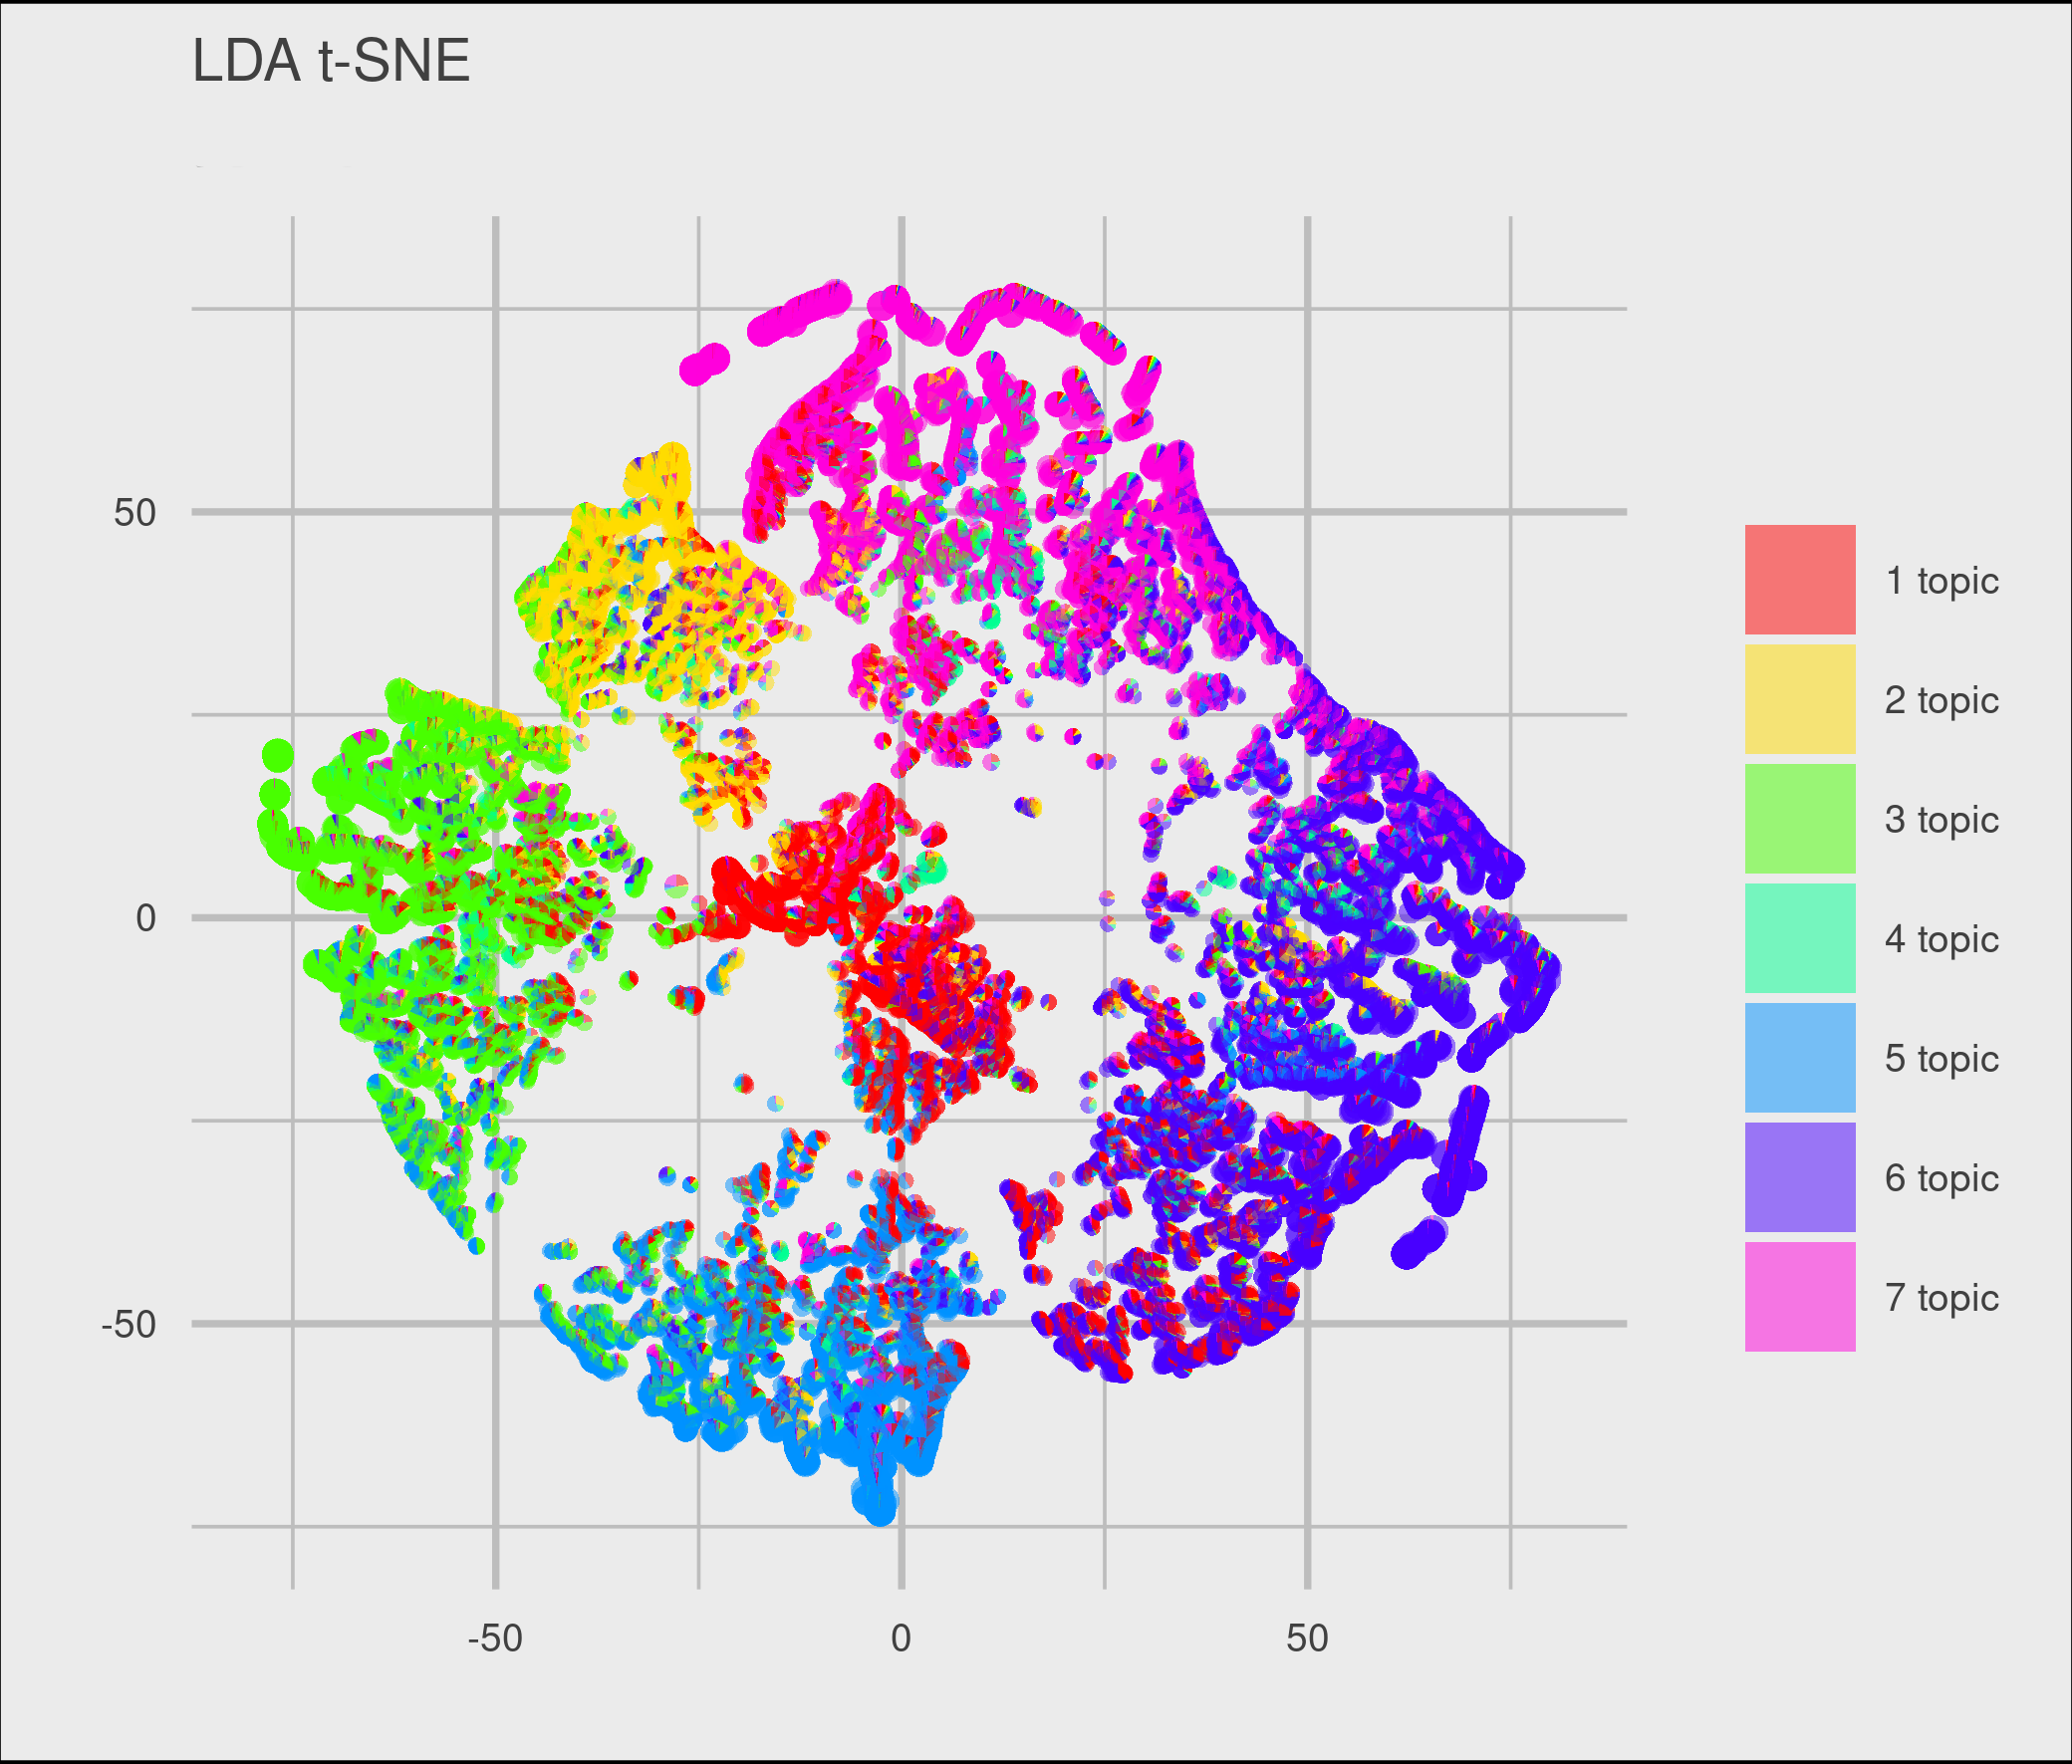
\includegraphics[width = 0.48\textwidth]{scatterpie2_mod.png}
                \caption{t-SNE of LDA model}
                \label{fig:tsne}
            \end{figure}
            
            Every circle in the plot is a pie chart displaying topics proportions in the document, it's size is proportional to the probability of the most frequent topic, while their position are the outcome of projection. For matter of clarity we decide to show only the topics having the highest probability greater than $0.5$: excluding the most undecided documents, we observe that topics clusters are well separated. We can't infer too much from the chart, especially about distances between clusters, but the fact the documents are well clusterized suggests us a good exclusivity value in our model. We also observe we missed Topic 4, and situation doesn't improve lowering the threshold: we'll see we have a high uncertainty about this topic. Finally we notice that applying lemmatization, instead of stemming, in a pre-processing step brigs us to overlapping topics in intertopic map, so we choose not to perform it. The exclusivity between topics is also supported by calculating Jaccard and Kullback–Leibler distance matrixes between them. All these charts are available in the \cite{GitHub_NR} repository.\\
            Now, we want to analyze how are LDA topics correlated with positive and negative reviews, with a $95\%$ confidence interval. Next, we try to make sense of them experimenting manually with some values of $\lambda$. As we can see in Figure \ref{fig:lda_total}, in which we analyze the percentage of each topic in positive reviews, only the third topic can't be classified properly and we have a quite large CI in the fourth. In addition to this visualization, we also build the same chart for each drug class. Let us try to make some inference and draw conclusions about topic-words distributions and how they appear in positive or negative reviews.

            \begin{figure}[!ht]
                \centering
                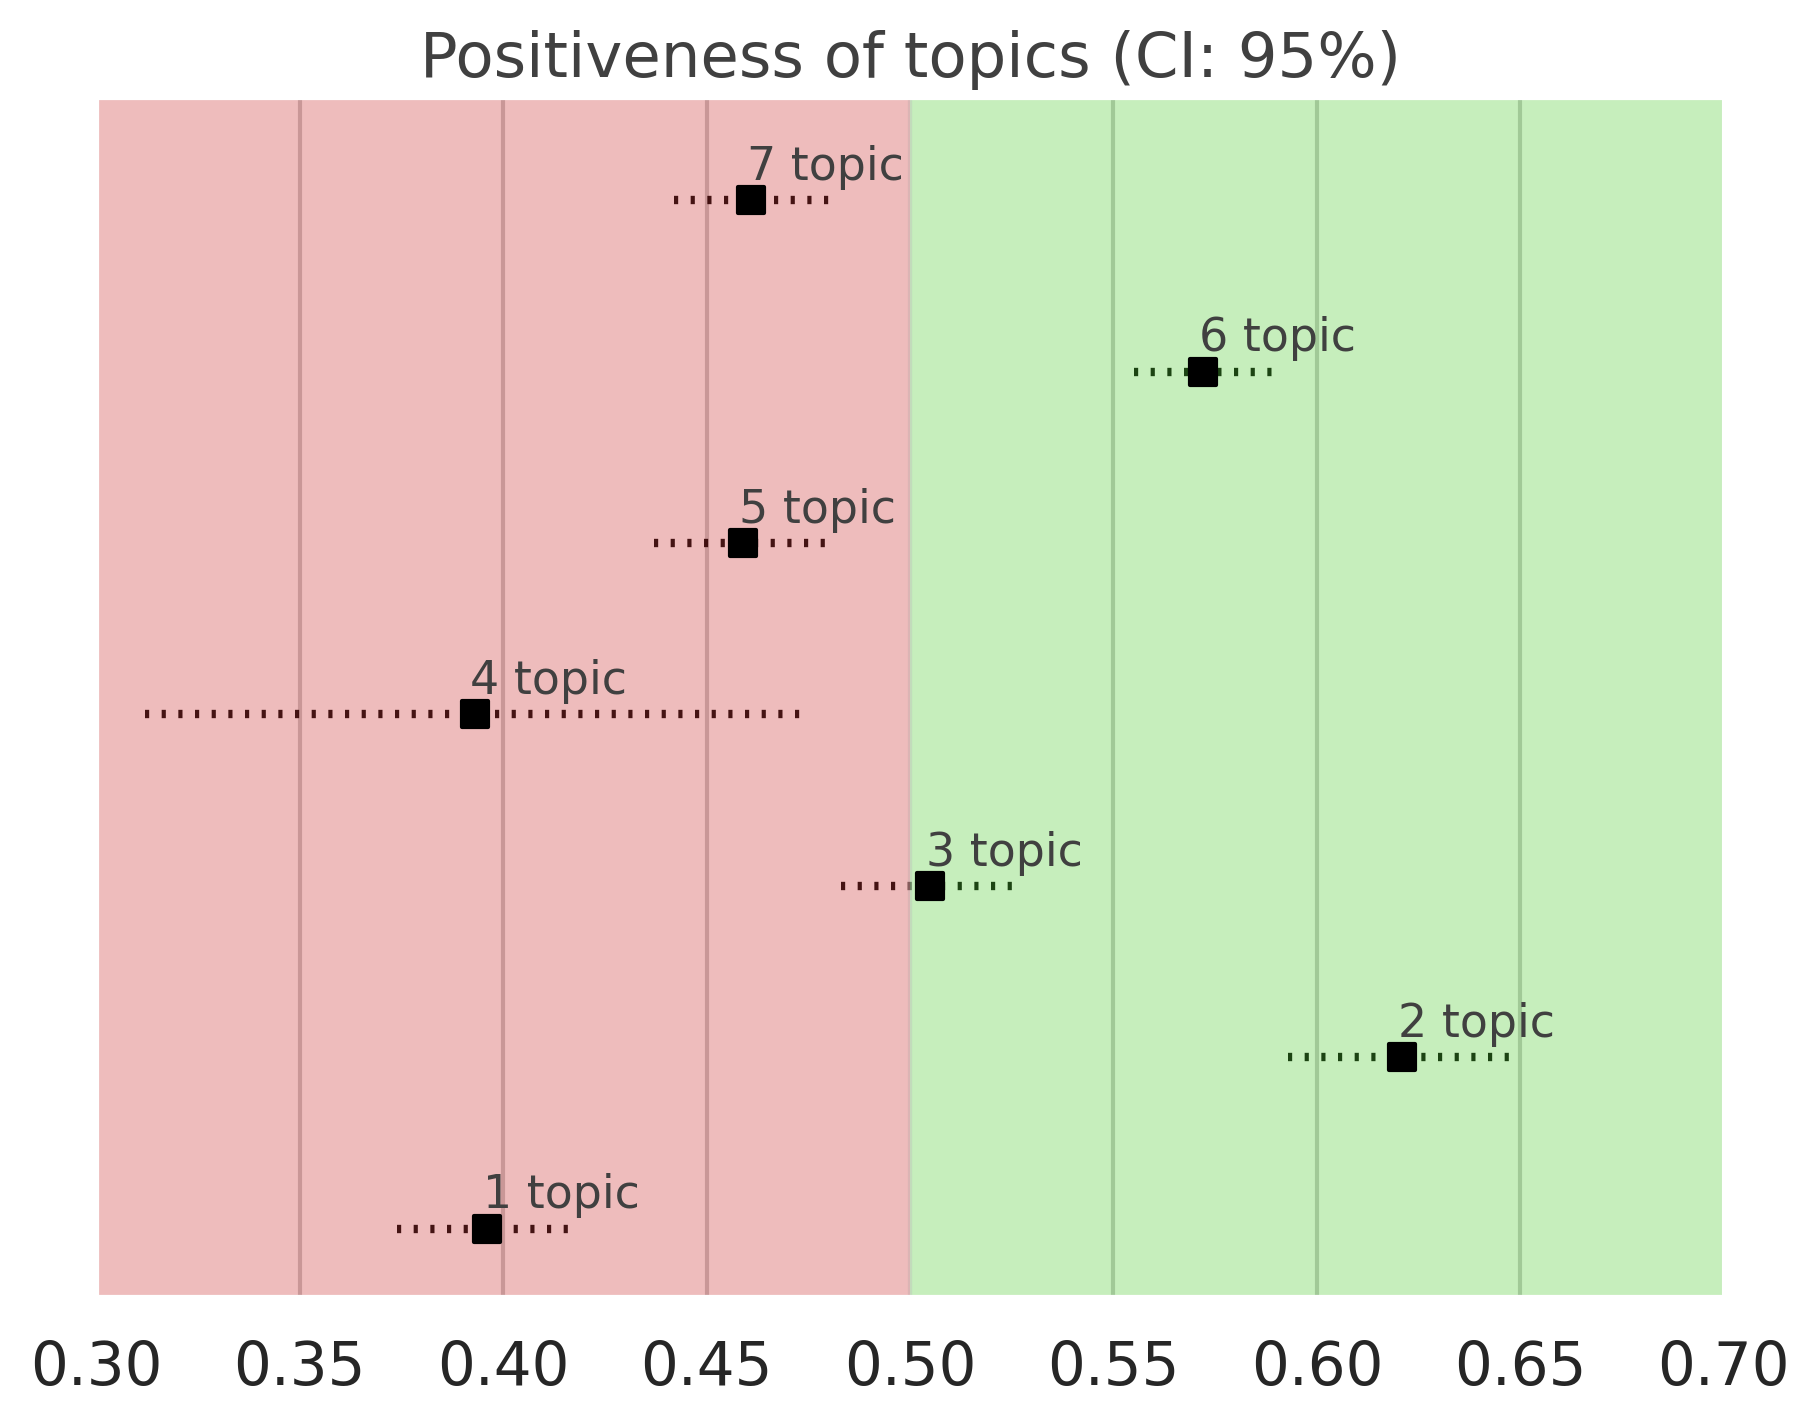
\includegraphics[width = 0.48\textwidth]{LDA_positivity_total.png}
                \caption{Ratio of positiveness of LDA topics, with $95\%$ CI}
                \label{fig:lda_total}
            \end{figure}

            There are 7 topics:
            \begin{enumerate}[label=\textbf{[\arabic*]}]
                \item This topic speaks about panic attacks, anxiety and depression. It's negatively linked with psychiatric drugs but also analgesics and anorexiants. One hypothesis is that these drugs don't properly heal the disease.
                \item It regards side effects and it's negatively associated with psychiatry but positively with contraceptives. Contraceptives side effects are indeed a hot topic in women.
                \item This topic is not significant in almost all classes but the problem it raises finds explanation in laxatives: they may bring cramps and bleed.
                \item Fourth topic tells us about migraine in people that take anorexiants or antipsychotics, especially during sleep or at work. We don't really know if this side effects derives from the drug or the disease.
                \item This hot topic speaks about gaining weight. It is positive in patients taking incretine mimetics (i.e. antidiabetes drugs) but negative in antidepressants, antipsychotics and contraceptives.
                \item Theme here is difficult to be associated with a particular problem, and varies from class to class. It seems to speak about how and when to take prescribed medicines.
                \item Last topic gives us information about the sensitivity of patients to economical costs of drugs. Its behaviour is oscillating among classes, but we can say it's felt as negative in contraceptive. Maybe people desire it to be free.
            \end{enumerate}
            Unfortunately, smoking cessation agents aren't linked to any positive or negative significant topic.\\

            \textbf{STM}\\
            For STM model we just compute metrics: we have an average semantic coherence of $-426.796$ and an exclusivity of $9.528$.\\
            Now, since STM model has too many possible topics to be analyzed, we just concentrate our thought on aspects regarding time. In fact, the year in which each review was written may suggest us important behavioural --- or drug formulation --- changes in time. Doing this we hope to contextualize our previous observations. Unfortunately, we performed STM in order to obtain more specialized topics that may enlighten class-specific problems. However, too general and not well interpratable topics prevailed among classes, just highlighting common aspects. We could finally state that LDA performs better in giving useful insights, specifically on single classes.\\
            
            The 7 topics are:
            \begin{enumerate}[label=\textbf{[\arabic*]}]
                \item It speaks about depression and panics attacks, as well as first topic in LDA, but also body weight and itch. Anyway, it's importance decreased in last years.
                \item Patients leverage this topic to inform us about mood disorders and addiction. This topic is less discussed in last years, thought.
                \item It's negative and its importance arose a lot recently. We may detect drugs side effects in this topic.
                \item Fourth topic is significantly associated with negative reviews: it regards headache, bleeding and pain depending on class. It's importance persisted in years. 
                \item This topic reveals how positively drugs helped patients at work or while sleeping.
                \item Similarly to fourth topic, this one speaks of migraine. This time, however, its prevalence decreased over years.
                \item This last topic may suggest us anorexiants improved their effectiveness in the last years, but it's also associated with skin in contraceptives and with falling asleep in anxiolytics.
            \end{enumerate}
            Leveraging the shiny app we could either explore other charts such as correlation between topics or see how some words of one topics are also present in an other topic. Still, these aspects turned out to be not really informative for our research question.
            
            
    \section{Sentiment Analysis}
      
            
        \subsection{Pre-processing}
         Each drug review is been cleaned first by defining a function consists in several steps concerning the special characters removal and multiple spaces, dots and pattern replace. Next, the cleaned reviews are processed with the Python Natural Language Toolkit. In this step, stopwords are removed and single word stemmed by Snowball Stemmer to reduce an inflected word down to its word stem. Afterwards we use Textblob module to give the sentiment polarity of the review. This polarity is given to both the cleaned reviews and the ones without removing the stop words and using snowball stemmer. TextBlob’s output for a polarity task is a float within the range $[-1.0, 1.0]$ where $-1.0$ is a negative polarity and $1.0$ is positive.\\ 
         For giving a score based on the sentiment expressed by words, TextBlob and VADER are two of the most widely used Sentiment Analysis Python libraries. Both of them are lexicon-based methods that work by mapping words and sentiment; as a result, the sentiment of a sentence is the aggregation of the sentiment of each term.
         We prefer to apply Textblob instead of VADER to reach our research question because VADER is usually focused on social media. Therefore, it puts a lot of effort into identifying the sentiments of content that typically appear on social media, such as emojis, repetitive words, and punctuations (exclamation marks, for example), so that we choose Textblob polarity to analyze drug patients reviews.\\
         To capture the complex nuances of language and provide a more accurate analysis of sentiment in text, we create new features engineering. The performance of Text Classification models largely depends on the quality and relevance of the features used. Hence, by creating new features that are more relevant and informative, we can improve the accuracy of the models.
         The final step of pre-processing procedure is to use the Label Encoder to change the categorical values of Drug Names and the Conditions in to numerical values for the machine learning modelling.
 
        \subsection{Models}
        After exploring different topic classification algorithms, we decide to implement and compare LightGBM, Logistic Regression and Gaussian Naive Bayes algorithms.
        The dataset is split in training ($0.8$) and test ($0.2$) sets, randomly. All the models are trained on the training set and have to classify the review sentiment defined by the polarity function by using the other features as covariates.\\
        LightGBM is a gradient boosting framework that uses treebased learning algorithms. In this case, the model is instantiated with certain hyperparameters, including the number of estimators ($10.000$), learning rate ($0.10$), number of leaves ($30$), and other parameters that impact the model's performance. The classifier is used to predict the sentiment of new drug reviews based on the patterns it has learned from the training data.\\
        Logistic Regression is a statistical method used for predicting binary outcomes, in which the dependent variable can have only two values (either $0$ or $1$) that, in this context of drug review classification, are the possible polarity scores indicate positiveness and negativeness. The model is instantiated with a "liblinear" solver: a popular optimization algorithm that works well for small and medium-sized datasets. The "liblinear" solver uses a modified version of the Coordinate Descent algorithm, where it solves the optimization problem over a sequence of values for the regularization parameter.\\
        The last model we choose to implement in order to classify the reviews based on the polarity reviews score is the Gaussian Naive Bayes Classifier, which is a variant of the Naive Bayes algorithm used for classification tasks. GaussianNB is a function of the sklearn library in Python, which creates an instance of the Gaussian Naive Bayes algorithm. So that, the Gaussian Naive Bayes algorithm assumes that each feature follows a Gaussian distribution, and that the features are independent of one another.
        
        \subsection{Evaluation}
        We consider accuracy, AUC and ROC curve as metrics for evaluate the model performance on test set. 
        
        \begin{equation*}
            Accuracy = \frac{TP + TN}{TP + TN + FP + FN}
        \end{equation*}
        
        where TP (True Positives) represents the number of instances correctly predicted as positive, TN (True Negative) represents the number of instances correctly predicted as negative, FP (False Positives) represents the number of instances wrongly predicted as positive, and FN (False Negatives) represents the number of instances wrongly predicted as negative.
        AUC (Area Under the Curve) and ROC (Receiver Operating Characteristic) curve are useful for performance evaluation when classifying drug reviews. These metrics are commonly used in machine learning and data mining for evaluating the performance of binary classifiers. In this case, the classifier would be used to categorize drug reviews as positive, negative, or neutral.\\
        The ROC curve is a graph that shows the tradeoff between sensitivity and specificity for different classification thresholds. A classifier with a higher AUC value, that is, closer to $1.0$, indicates that it has better discriminative power to correctly identify positive and negative reviews.
        We notice that the model which have the highest accuracy value ($0.8$) and AUC nearest to $1.0$ ($0.8$) is the LightGBM.
        
        \begin{figure}[!ht]
                \centering
                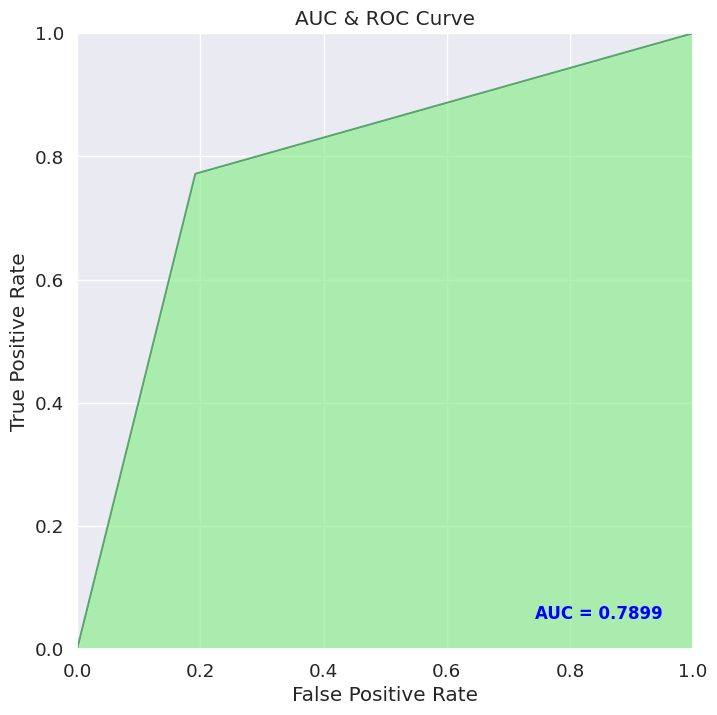
\includegraphics[width = 0.48\textwidth]{AUC1.png}
                \caption{AUC of LightGBM performance}
                \label{fig:auc1}
            \end{figure}

    \section{Conclusions}
        Managing with patients reviews in order to classify what they say and to extract their feelings are not easy tasks. However, using different algorithms for Topic Modelling allowed us to discriminate topics and also discover patterns with a different granularity levels. Indeed, LDA performs better in giving useful insights, while STM seems to give more general information. Moreover, the models we implemented for Sentiment Analysis have revealed to quantify the emotions explained by the features. In this way, we forced data and associated a polarity measure to what patients feel and we obtained different results. LightGBM seemed to be the best model in classifying new reviews using patients sentiment score. 
    

 
    %	BIBLIOGRAPHY
    
    \addcontentsline{toc}{section}{References}
	\renewcommand\refname{References}
        {\footnotesize
	\begin{thebibliography}{99}

             \bibitem[Gräßer et al., 2018]{Graber}F. Gräßer, S. Kallumadi, H. Malberg and S. Zaunseder (2018). \textit{Aspect-Based Sentiment Analysis of Drug Reviews Applying Cross-Domain and Cross-Data Learning}. In \textit{Proceedings of the 2018 International Conference on Digital Health}
 
             \bibitem[He et al., 2020]{drug} L. He, D. Han, X. Zhou and Z. Qu (2020). \textit{The Voice of Drug Consumers: Online Textual Review Analysis Using Structural Topic Model}
    
             \bibitem[Hu et al., 2019]{hotel} N. Hu, T. Zhang, B. Gao and I. Bose (2019). \textit{What do hotel customers complain about? Text analysis using structural topic model}
             
             \bibitem[Rossetti et al., 2015]{tourism} M. Rossetti, F. Stella and M. Zanker (2015). \textit{Analyzing user reviews in tourism with topic models}
            
             \bibitem[Uddin et al., 2022]{drug2} M. N. Uddin, M. F. B. Hafiz and S. Hossain (2022). \textit{Drug Sentiment Analysis using Machine Learning Classifiers}
    
             \bibitem[Syed et al., 2017]{Syed} S. Syed and M. Spruit (2017). \textit{Full-Text or Abstract? Examining Topic Coherence Scores Using Latent Dirichlet Allocation}
    
             \bibitem[Mimno et al., 2011]{Mimno} D. Mimno, H. M. Wallach, E. Talley and M. Leenders (2011). \textit{Optimizing Semantic Coherence in Topic Models}
    
             \bibitem[Sievert et al., 2014]{Sievert} C. Sievert and K. Shirley (2014). \textit{LDAvis: A method for visualizing and interpreting topics}
             
             \bibitem[Choco, 2023]{Kaggle_choco} Choco, (2023). URL:\\ https://www.kaggle.com/code/chocozzz/recommendation-medicines-by-using-a-review/notebook/
             
             \bibitem[GitHub]{GitHub_NR} N. Rocchi, G. Gravina (2023). URL: \\https://github.com/Niccolo-Rocchi/Text-Mining-Project/
             
             \bibitem[Nagy, 2018]{Kaggle_Peter} P. Nagy (2018). URL: \\https://www.kaggle.com/code/ngyptr/python-nltk-sentiment-analysis/notebook/
    
            \bibitem[Blei et al., 2003]{LDA} David M. Blei, Andrew Y. Ng, M. I. Jordan (2003). \textit{Latent Dirichlet Allocation}
    
            \bibitem[Drugs.com]{drugs.com} Drugs.com site. URL: https://www.drugs.com/

            

            

        \end{thebibliography}
        }

\end{document}
